% \iffalse
\let\negmedspace\undefined
\let\negthickspace\undefined
\documentclass[journal,12pt,twocolumn]{IEEEtran}
\usepackage{cite}
\usepackage{amsmath,amssymb,amsfonts,amsthm}
\usepackage{algorithmic}
\usepackage{graphicx}
\usepackage{textcomp}
\usepackage{xcolor}
\usepackage{txfonts}
\usepackage{listings}
\usepackage{enumitem}
\usepackage{mathtools}
\usepackage{gensymb}
\usepackage{comment}
\usepackage[breaklinks=true]{hyperref}
\usepackage{tkz-euclide} 
\usepackage{listings}
\usepackage{gvv}                                        
\def\inputGnumericTable{}                                 
\usepackage[latin1]{inputenc}                                
\usepackage{color}                                            
\usepackage{array}                                            
\usepackage{longtable}                                       
\usepackage{calc}                                             
\usepackage{multirow}                                         
\usepackage{hhline}                                           
\usepackage{ifthen}                                           
\usepackage{lscape}
\newtheorem{theorem}{Theorem}[section]
\newtheorem{problem}{Problem}
\newtheorem{proposition}{Proposition}[section]
\newtheorem{lemma}{Lemma}[section]
\newtheorem{corollary}[theorem]{Corollary}
\newtheorem{example}{Example}[section]
\newtheorem{definition}[problem]{Definition}
\newcommand{\BEQA}{\begin{eqnarray}}
\newcommand{\EEQA}{\end{eqnarray}}
\newcommand{\define}{\stackrel{\triangle}{=}}
\theoremstyle{remark}
\newtheorem{rem}{Remark}
\begin{document}

\bibliographystyle{IEEEtran}
\vspace{3cm}

\title{CE-25}
\author{EE23BTECH11063 - Vemula Siddhartha}
\maketitle
\newpage
\bigskip

\renewcommand{\thefigure}{\theenumi}
\renewcommand{\thetable}{\theenumi}
\textbf{Question}:\\
The following function is defined over the interval $[-L,L]$:
    $$f\brak{x}=px^4+qx^5$$
It is expressed as a Fourier series,
    $$f\brak{x}=a_0+\sum_{n=1}^{\infty}\cbrak{a_n\sin\brak{\frac{\pi n x}{L}}+b_n\cos\brak{\frac{\pi n x}{L}}}$$
which options amongst the following are true?
\begin{enumerate}[label=(\alph*)]
    \item $a_n$, $n=1,2,..,\infty$ depend on $p$
    \item $a_n$, $n=1,2,..,\infty$ depend on $q$
    \item $b_n$, $n=1,2,..,\infty$ depend on $p$
    \item $b_n$, $n=1,2,..,\infty$ depend on $q$
\end{enumerate}
\textbf{Solution:}\\
% %\fi
% \begin{align}
%     f\brak{x}=a_0+\sum_{n=1}^{\infty}\cbrak{a_n\sin\brak{\frac{\pi n x}{L}}+b_n\cos\brak{\frac{\pi n x}{L}}}\label{eq:GATE_CE25_1}
% \end{align}
% Finding the Fourier Coefficient $a_0$,
% \begin{align}
%     a_0&=\frac{1}{2L}\int_{-L}^{L}f\brak{x}\;dx\\
%     &=\frac{1}{2L}\int_{-L}^{L}\brak{px^4+qx^5}\;dx\\
%     &=\frac{1}{2L}\brak{2\int_{0}^{L}px^4\;dx+0}\\
%     &=\frac{p}{L}\frac{x^5}{5}\Bigg|_{-L}^{L}\\
%     \implies a_0&=\frac{2pL^4}{5}
% \end{align}
% Finding the Fourier Coefficients $a_n$,
% \begin{align}
%     a_n&=\frac{1}{L}\int_{-L}^{L}f\brak{x} \sin\brak{\frac{\pi n x}{L}}\;dx\\
%     &=\frac{1}{L}\int_{-L}^{L}\brak{px^4+qx^5}\sin\brak{\frac{\pi n x}{L}}\;dx\\
%     &=0+\frac{1}{L}\int_{-L}^{L}qx^5\sin\brak{\frac{\pi n x}{L}}\;dx
% \end{align}
% \begin{align}
%     &=-\frac{q}{\pi n}\brak{x^5\cos\brak{\frac{\pi n x}{L}}}+\frac{5qL}{\brak{\pi n}^2}\brak{x^4\sin\brak{\frac{\pi n x}{L}}}\notag\\
%     &\;\;\;+\frac{20qL^2}{\brak{\pi n}^3}\brak{x^3\cos\brak{\frac{\pi n x}{L}}}-\frac{60qL^3}{\brak{\pi n }^4}\brak{x^2\sin\brak{\frac{\pi n x}{L}}}\notag\\
%     &\;\;\;-\frac{120qL^4}{\brak{\pi n}^5}\brak{x\cos\brak{\frac{\pi n x}{L}}}+\frac{120qL^5}{\brak{\pi n}^6}\sin\brak{\frac{\pi n x}{L}}\Bigg|_{-L}^{L}\\
%     &=-\frac{2q}{\pi n}\brak{L^5\cos\brak{\pi n }}+\frac{40qL^2}{\brak{\pi n}^3}\brak{L^3\cos\brak{\pi n }}\notag\\
%     &\;\;\;-\frac{240qL^4}{\brak{\pi n}^5}\brak{L\cos\brak{\pi n}}\\
%     \implies a_n&=\brak{-1}^{n+1}\brak{2qL^5}\brak{\frac{1}{\pi n}-\frac{2}{\brak{\pi n}^3}+\frac{120}{\brak{\pi n}^5}}
% \end{align}
% Finding the Fourier Coefficients $b_n$,
% \begin{align}
%     b_n&=\frac{1}{L}\int_{-L}^{L}f\brak{x} \cos\brak{\frac{\pi n x}{L}}\;dx\\
%     &=\frac{1}{L}\int_{-L}^{L}\brak{px^4+qx^5}\cos\brak{\frac{\pi n x}{L}}\;dx\\
%     &=\frac{1}{L}\int_{-L}^{L}px^4\cos\brak{\frac{\pi n x}{L}}\;\;dx+0\\
%     &=\frac{p}{\pi n}\brak{x^4\sin\brak{\frac{\pi n x}{L}}}+\frac{4pL}{\brak{\pi n}^2}\brak{x^3\cos\brak{\frac{\pi n x}{L}}}\notag\\
%     &\;\;\;-\frac{12pL^2}{\brak{\pi n}^3}\brak{x^2\sin\brak{\frac{\pi n x}{L}}}-\frac{2pL^3}{\brak{\pi n}^4}\brak{x\cos\brak{\frac{\pi n x}{L}}}\notag\\
%     &\;\;\;+\frac{24pL^4}{\brak{\pi n }^5}\sin\brak{\frac{\pi n x}{L}}\Bigg|_{-L}^{L}\\
%     &=\frac{8pL}{\brak{\pi n}^2}\brak{L^3\cos\brak{\pi n}}-\frac{2pL^3}{\brak{\pi n}^4}\brak{L\cos\brak{\pi n}}\\
%     \implies b_n&=\brak{-1}^n\brak{2pL^4}\brak{\frac{4}{\brak{\pi n}^2}+\frac{1}{\brak{\pi n}^4}}
% \end{align}
The complex exponential Fourier Series of $f\brak{x}$ is,
\begin{align}
    f\brak{x}&=\sum_{-\infty}^{\infty}c_ne^{j\frac{\pi nx}{L}}\\
    c_n&=\frac{1}{2L}\int_{-L}^{L}f\brak{x}e^{-j\frac{\pi n x}{L}}\;dx\\
    &=\frac{1}{2L}\int_{-L}^{L}\brak{px^4+qx^5}e^{-j\frac{\pi n x}{L}}\;dx\\
    &=\frac{pL^4}{2}\brak{e^{j\pi n}-e^{-j\pi n}}\brak{\frac{1}{j\pi n}+\frac{12}{\brak{j\pi n}^3}+\frac{24}{\brak{j\pi n}^5}}\notag\\
    &\;\;\;-\frac{pL^4}{2}\brak{e^{j\pi n}+e^{-j\pi n}}\brak{\frac{4}{\brak{j\pi n}^2}+\frac{24}{\brak{j\pi n}^4}}\notag\\
    &\;\;\;-\frac{qL^5}{2}\brak{e^{j\pi n}+e^{-j\pi n}}\brak{\frac{1}{j\pi n}+\frac{20}{\brak{j\pi n}^3}+\frac{120}{\brak{j\pi n}^5}}\notag\\
    &\;\;\;+\frac{qL^5}{2}\brak{e^{j\pi n}-e^{-j\pi n}}\brak{\frac{5}{\brak{j\pi n}^2}+\frac{60}{\brak{j\pi n}^4}+\frac{120}{\brak{j\pi n}^6}}\\
    c_n&=0-\brak{pL^4}\brak{-1}^n\brak{-\frac{4}{\brak{\pi n}^2}+\frac{24}{\brak{\pi n}^4}}\notag\\
    &\;\;\;-\brak{qL^5}\brak{-1}^n\brak{-\frac{j}{{\pi n}}+\frac{20j}{\brak{\pi n}^3}-\frac{120j}{\brak{\pi n}^5}}+0
\end{align}
We know,
\begin{align}
    f\brak{x}=a_0+\sum_{n=1}^{\infty}\cbrak{a_n\sin\brak{\frac{\pi n x}{L}}+b_n\cos\brak{\frac{\pi n x}{L}}}
\end{align}
% Here,
% \begin{align}
%     a_n&=\frac{c_n-c_{-n}}{2j}\\
%     b_n&=\frac{c_n+c_{-n}}{2}
% \end{align}
Finding the Fourier Coefficient $a_0$,
\begin{align}
    a_0&=c_0\\
    \implies a_0&=\frac{1}{2L}\int_{-L}^{L}f\brak{x}\;dx\\
    &=\frac{1}{2L}\int_{-L}^{L}\brak{px^4+qx^5}\;dx\\
    &=\frac{pL^4}{5}
\end{align}
Finding the Fourier Coefficients $a_n$,
\begin{align}
    a_n&=\frac{c_{-n}-c_n}{j}\\
    \implies a_n&=\brak{-2qL^5}\brak{-1}^{n}\brak{\frac{1}{\pi n}-\frac{2}{\brak{\pi n}^3}+\frac{120}{\brak{\pi n}^5}}
\end{align}
Finding the Fourier Coefficients $b_n$,
\begin{align}
    b_n&=c_n+c_{-n}\\
    \implies b_n&=\brak{2pL^4}\brak{-1}^n\brak{\frac{4}{\brak{\pi n}^2}-\frac{24}{\brak{\pi n}^4}}
\end{align}
Hence, options \brak{\text{b}} and \brak{\text{c}} are correct.
\begin{figure}[h!]
    \centering
    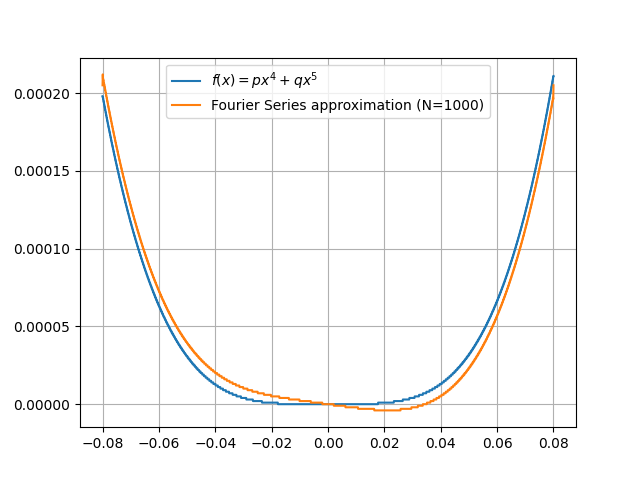
\includegraphics[width=\linewidth]{figs/Figure_1.png}
    \caption{Fourier Series Approximation of $f\brak{x}$ for $p=5$, $q=2$, $L=0.08$}
\end{figure}
\end{document}
